\documentclass{article}
\usepackage[utf8]{inputenc}
\usepackage[T1]{fontenc}
\usepackage{newtxtext,newtxmath}
\usepackage{graphicx}
\usepackage{float}
\usepackage{hyperref}

\title{ELK330\_Lab3}
\author{Aksel Fosså}
\date{October 2026}

\begin{document}
%--------------------------------------------------
\maketitle
\section{Prosjekttittel}
Jeg har valgt: Kortslutningsanalyse og vernkoordinering

%-----------------------------------------------------
\section{Problemstilling og mål}
\subsection{Problem}
Kortslutninger i kraftsystemer kan føre til store strømmer som skader utstyr og gir strømbrudd i strømforsyningen. Vernsystemer må derfor oppdage feil og koble ut riktig del av nettet.

\subsection{Relevans}

Kortslutningsanalyse og vernkoordinering er grunnleggende oppgaver ved planlegging og drift av elektriske kraftsystemer. Feil koordinering kan føre til unødvendige utkoblinger eller manglende beskyttelse av utstyr.

\subsection{Spørsmål}
\begin{itemize}
    \item Hvordan beregnes kortslutningsstrømmer i et distribusjonsnett?
    \item Hvordan påvirker feilplassering og type feil kortslutningsnivåene?
    \item Hvordan kan vern innstilles for å oppnå selektiv utkobling?
    \item Hvilke utfordringer oppstår ved koordinering av flere vern i samme nett?
\end{itemize}

\subsection{Hovedmål}
Å undersøke kortslutningsnivåer i et distribuert kraftsystem og evaluere vernkoordinering mellom flere vern.

\subsection{Delmål}
\begin{itemize}
    \item Utvikle en modell av et enkelt distribusjonsnett.
    \item Gjennomføre kortslutningsanalyser for ulike feil.
    \item Analysere vernrespons ved forskjellige feilscenarier.
    \item Vurdere om vernene fungerer selektivt.
\end{itemize}

\subsection{Forventede resultater}
\begin{itemize}
    \item Beregnede kortslutningsstrømmer.
    \item Sammenligning av ulike feilscenarier.
    \item Forslag til verninnstillinger.
    \item Vurdering av selektivitet.
\end{itemize}


%---------------------------------------------------------
\section{Faglig bakgrunn og litteratursøk}
Dette er referanser jeg har funnet og så er en hel referanse liste rett under:\cite{relayreview}\cite{abb_coordination}\cite
{glover}\\
\\
For å finne informasjon har jeg brukt Google, IEEE Xplore og andre ulike faglige nettsider. Jeg har også brukt boken \textit{Power System Analysis and Design} og andre kilder som handler om kortslutningsanalyse og vernkoordinering.
\bibliographystyle{splncs04}
\bibliography{biblio} 

%--------------------------------------------------------
\newpage
\section{Modellambisjon}
\subsection{Kompleksitet}
Middels\\
Modellen inneholder flere komponenttyper som transformator, linjer, laster og vern, men representerer ikke hele transmisjonssystemer.

\subsection{Integrasjon}
Lav til middels\\
Fokus ligger på det elektriske kraftsystemet og vernsystemet. Modellen integrerer ikke markedsmodeller, kommunikasjonsnett eller andre infrastruktursystemer.

\subsection{Begrunnelse}
Prosjektet fokuserer på kraftsystemanalyse og beskyttelse. Dette krever en modell med tilstrekkelig detaljnivå for beregning av kortslutningsstrømmer og vernrespons, men uten unødvendig kompleksitet.

\subsection{Antakelser og forenklinger}
\begin{itemize}
    \item Symmetrisk trefasesystem
    \item Konstante impedanser
    \item Ideelle vernkarakteristikker
    \item Stasjonær driftstilstand før feil
    \item Ingen transient analyse
    \item Ingen temperaturavhengighet
    \item Begrenset modell av vernlogikk
\end{itemize}

\subsection{Balanse mellom ambisjoner og arbeidsomfang}
Jeg plannleger å lage en modell som er ikke er for detaljert, men har nok komponenter til å kunne studere kortslutningsstrømmer og vernrespons. Det vil derfor bli fokusert på et begrenset distribusjonsnett med et mindre antall komponenter og feil.

\newpage
%---------------------------------------------------
\section{Gjennomføringsplan}
\subsection{Typer Feil}
\begin{itemize}
    \item trefase feil
    \item enfase og jord feil
    \item tofase feil
\end{itemize}
\subsection{Scenarioer}
\begin{itemize}
    \item Feil nær transformator
    \item Feil midt på linje
    \item Feil ved enden av linje
\end{itemize}
\subsection{Interessante resultater}
\begin{itemize}
    \item Maksimal kortslutningsstrøm
    \item Minimal kortslutningsstrøm
    \item Vernenes utkoblingstid
\end{itemize}

\subsection{Timebruk}
\begin{itemize}
    \item Litteratursøk: 5 timer
    \item Modellering: 10 timer
    \item Simulering: 8 timer
    \item Analyse: 7 timer
    \item Rapport: 10 timer
\end{itemize}
Time bruken er antagelser det kan fort ta lenger og mindre tid på de forskjellige delene. Jeg vet ikke hvor mye tid jeg har til gode med andre fag ennå, men jeg føler jeg kan bruke sette av rundt 15-20timer i uken til raporten.

%-------------------------------------------------------------------------------
\section{Formelle krav}
\subsection{Figur}
\begin{figure}[H]
    \centering
    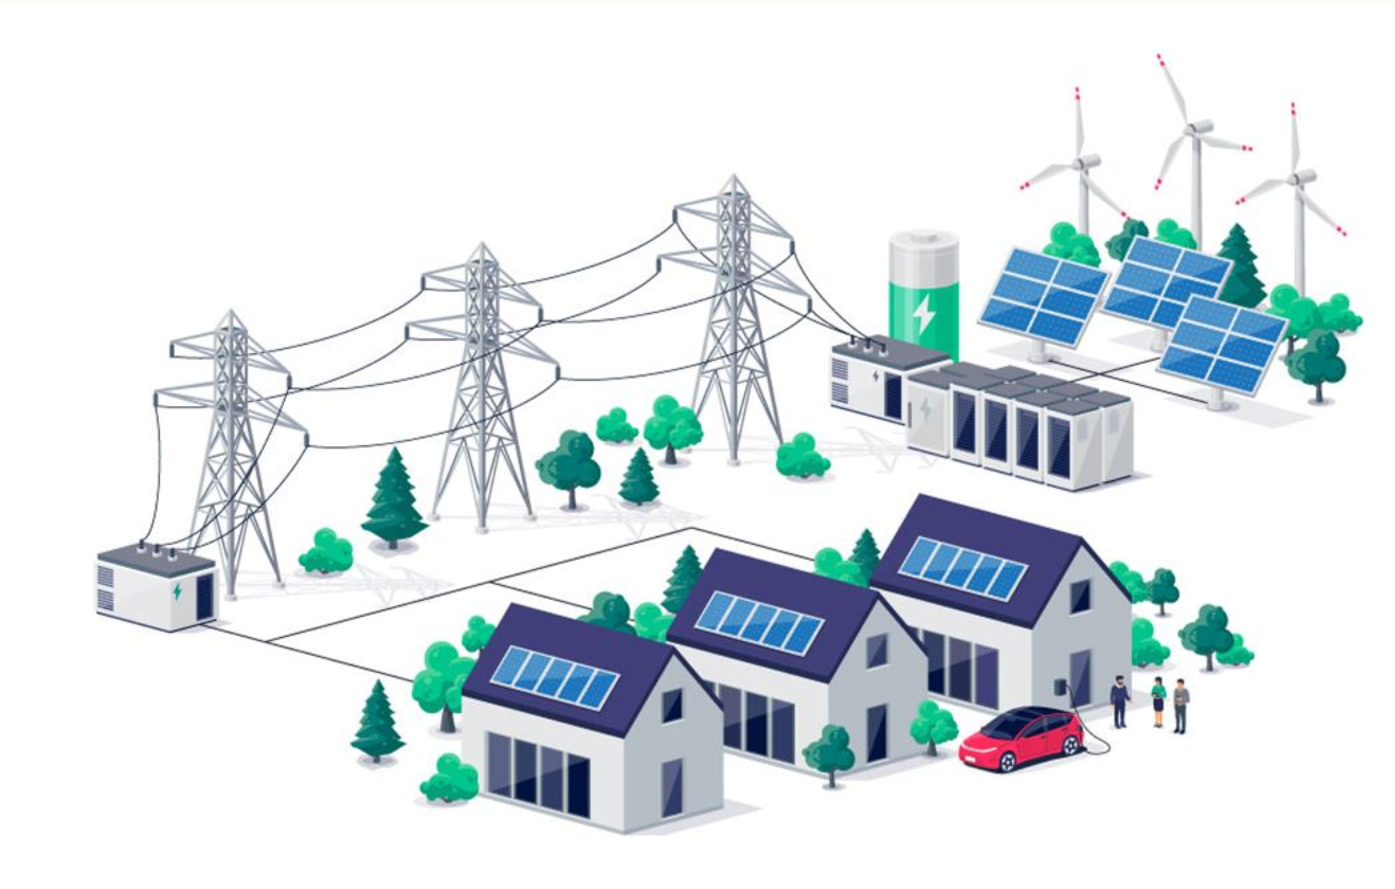
\includegraphics[width=0.5\linewidth]{Eksempel_fig.png}
    \caption{Eksempel bilde}
    \label{fig:Nett}
\end{figure}
\subsection{Tabel}

\begin{table}[H]
    \centering
    \begin{tabular}{cc}
        En-fase & Tre-fase\\
        230V & 400V\\
    \end{tabular}
    \caption{Eksempel Tabell}
    \label{tab:Tabel}
\end{table}

Jeg viser hvordan jeg kan referer til en Figur~\ref{fig:Nett} og Tabell~\ref{tab:Tabel}

\section{Ønsker innleveringsform}
Jeg ønsker å lever rapporten som pdf skrevet i latex kode
%-------------------------------------------------------------------------------
\end{document}
